\chapter{Background \& Objectives}

\section{Overview}
This project is designed to examine the properties of mapping higher dimensional data onto a lower dimensional representation using manifold learning techniques. More specifically the project will aim to provide a study of using dimensionality reduction techniques on both real and synthetic \cite{bakic2002mammogram1, bakic2002mammogram2, bakic2003mammogram3} mammogram datasets to evaluate their relationship under the mapping.

The main goal of the project will be to produce a processing pipeline that loads and pre- processes mammograms from both real and synthetic datasets. Feature extraction methods can then be used to find relevant features within both of these datasets. Once features have been extracted dimensionality reduction techniques can be applied and the results visualised in a lower dimensional space. Visualisation of the results does not necessarily need to be limited to 2-3 dimensions. It is hoped that a clear pattern will be found between both the synthetic and real data with the results from both datasets appearing close to each other in the lower dimensional representation.

The choice of manifold learning algorithm and feature extraction techniques are the main components under consideration for this project. This will require further background reading and research to evaluate the best candidates for each of these components. Ideally the project should focus on feature extraction methods which are commonly used and well understood in mammogram analysis. A variety of different manifold learning approaches can then be applied to the extracted features to reduce the dimensionality of the resulting data and select only those features which are most relevant. There will also need to be careful consideration regarding what metrics are used to evaluate the quality of the results of these techniques.

The result of the project will be to provide an evaluation of the similarities and differences between the lower dimensional mappings produced from datasets. One aim is try to distinguish whether the differences are in agreement with the limitations discussed by the authors of the synthetic data. It would also be interesting to see how well the different classes of risk line up under a lower dimensional mapping of the two datasets and which features are selected using the dimensionality reduction techniques for each dataset. Could the knowledge gained be used to influence a radiologist’s perception of what features are important in a mammogram? Could it be used to provide information about how to build better mammogram models?

\section{Mammography}

Breast cancer is the leading cause of death among women and is the most common form of cancer found in women \cite{siegel2014cancer}. Early screening of breast cancer using mammography has been shown to reduce the mortality rate of women \cite{independent2012benefits, smith2014cancer}.

Mammography is the analysis of female breast tissue through the use of X-ray radiology with the goal of producing high resolution images of the structure within the female breast. The composition of the parenchymal patterns and tissue density revealed by in a mammographic evaluation can be used in the early detection of breast cancer.

Qualitatively speaking the composition of breast tissue can be split into four distinct categories. These are nodular densities (corresponding to Terminal Ductal Lobular Units (TDLUs), linear densities (corresponding to ducts, vessels, and fibrous strands), homogeneous, structureless densities (corresponding to fibrous supporting tissue), and radiolucent areas (corresponding to adipose tissue)\cite{tabar2005breast}. Typical markers used in the detection of cancer are the presence of clusters of micro-calcifications, masses, architectural distortions, breast density and parenchymal patterns \cite{sampat2005computer}.

There are two main projections of the breast used in X-ray mammography. These are known as craniocaudal (CC) and mediolateral oblique (MLO). The craniocaudal view is the "bottom-up" view of the breast and is the best method for visualising the medial aspect of breast tissue \cite{fischer2008breast}. The mediolateral oblique projection is a "side-on" view of the breast that provides maximum visualisation of the breast tissue in its entirety but is limited in its ability to visualise the inner breast tissue \cite{fischer2008breast}.

\subsection{Mammogram Acquisition}
The difference between high risk and low risk breasts is inherently small in mammograms due to the low level of tissue contrast between the two classes \cite{kopans1998breast}. Because of this the most essential part of mammographic imaging to ensure that a high contrast resolution is achieved in order to successfully capture the fine detail of the internal structures.

Mammopgraphic imaging has historically been carried using film but is now more commonly performed using digital mammography. Regardless of the medium the general technique for acquisition remains the same. The breast is placed on a plate between the X-ray tube and the detector. The breast is compressed from its normal conical shape onto the plate. This improves imaging by helping to ensure the X-ray attenuation through the breast tissue is as uniform as possible. 

Traditional film acquisition is hampered due to the film's sigmoid shaped response to x-ray exposure \cite{kopans1998breast}. This can lead to under or over exposure of the film which in turn leads to poor contrast. Digital mammography does not suffer from this issue because the response curve is essentially linear \cite{kopans1998breast}.


\subsection{Risk Assessment}
Mammograms provide a non-invasive means to assess the risk of a patient developing cancer. Several different systems have been developed to aid the classification of mammographic risk based on the parenchymal patterns visible through X-ray mammography.

\subsubsection{Wolfe}
The earliest attempt to classify mammographic risk using parenchymal patterns was suggested by Wolfe \cite{wolfe1976breast}. Wolfe proposed a classification system which split patients into four categories depending on the relative visible density of fat, ducts and connective tissue. The four categories are described, in order of lowest to highest risk, by Wolfe \cite{wolfe1976breast} as:

\begin{itemize}
	\item \textbf{N1} - Breast is mostly composed of fat with no visible ducts and very little amounts of dysplasia present. 
	\item \textbf{P1} - The parenchyma is primarily composed of fat with up to one quarter of the breast density being composed of visible ducts in the anterior position which may extend into a quadrant.
	\item \textbf{P2} - Breast indicates prominent duct pattern beyond one quarter of the breast that can occupy the entire parenchyma.
	\item \textbf{DY} - Breast is characterised by a severe increase in breast density and often appear as homogenous, missing the duct pattern present in P2 breasts.
\end{itemize}

\subsubsection{Boyd}
Boyd et al. \cite{boyd1995quantitative} proposed a quantitive assessment of risk based on increasing classes of mammographic density, known as the six class categories (SCC). These classes are based on the proportion of dense tissue relative to the area of the breast. The six classes are:

\begin{itemize}
	\item 0\%
	\item \textgreater 0 to \textless 10\% 
	\item 10 to \textless 25\% 
	\item 25 to \textless 50\%
	\item 50 to \textless 75\%
	\item $\geq$ 75\%
\end{itemize}

\subsubsection{Tab\'{a}r}
Tab\'{a}r et al. \cite{gram1997tabar} proposed a classification scheme which classifies a breast based on the percentage presence of the four building blocks of breast composition \cite{gram1997tabar, tabar2005breast}. The description of each of the five patterns is given as:

\begin{itemize}
	\item \textbf{Pattern I} - Breast corresponding to pattern I exhibit scalloped contours and cooper's ligaments with evenly scattered TDLU's.
	\item \textbf{Pattern II} - Complete fatty replacement of both
	\item \textbf{Pattern III} - Prominent retroareolar duct pattern and fatty involution.
	\item \textbf{Pattern IV} - Extensive linear and nodular densities present throughout the parenchyma.
	\item \textbf{Pattern V} - Homogeneous, structureless fibrosis with a convex contour.
\end{itemize}

\subsubsection{BI-RADS}
The Breast Imaging Reporting and Data System (BI-RADS) \cite{balleyguier2007birads} was developed by the American College of Radiology (ACR) in an attempt to standardise the lexicon used to describe mammography reports during standard screening. BI-RADS classifies the breast into four categories based on density \cite{balleyguier2007birads}.

\begin{enumerate}
	\item Fatty Breast (\textless10\% of dense tissue)
	\item Fibroglandular (10 - 49\% of dense tissue)
	\item Heterogeneously dense (49 - 90\% of dense tissue)
	\item Homogeneously dense (\textgreater 90\% of dense tissue)
\end{enumerate}

A radiologist will then classify the breast according to one of 7 categories after interpretation \cite{balleyguier2007birads}. These are one of:

\begin{itemize}
	\item Incomplete. Additional evaluation needed.
	\item Normal. 
	\item Typically benign.
	\item Probably benign. A shorter interval follow-up is recommended.
	\item Suspicious Abnormality. Biopsy considered.
	\item Highly suggestive of malignancy. Biopsy should be performed.
	\item Histologically proven malignancy.
\end{itemize}

\section{Features}
\label{sec:features}
Features are higher level descriptive abstractions computed from lower level structure such as points of intensity maxima, edges, and corners present within an image. Features can be thought of as the result of computing a descriptive property about an image from the intensity information contained within it. Hundreds of different types of features have been proposed in mammography. Broadly speaking, image features can be split into three distinct categories: shape (or morphological), intensity, and texture features. A brief review of some examples of each type are given in this section.


\subsection{Intensity Features}
Intensity features are possibly the simplest type of feature that can be detected from an image. Intensity features are simple descriptive statistics based on the grey-level histogram of an image or a patch of an image. Examples of such features are the mean, standard deviation/variance, skew, and kurtosis of the grey-level histogram of an ROI \cite{cheng2006approaches, christoyianni2000fast}.


\subsection{Shape Features}
Shape features are features which are based on the morphological properties of a region of interest (ROI) within an image. The ROI could either be a suspicious artefact present in the mammogram, such as a malignant or benign tumour or cluster of micro-calcifications \cite{cheng2006approaches}, or it could simply be a property present in the parenchymal structure of the mammogram (which is the approach used in this project) such as regions of high density tissue \cite{chen2013multiscale} or prominent linear structures \cite{zwiggelaar1996finding}.

Typical example of features extracted from shapes of an ROI are the area covered by the shape are the circularity or rectangularity of the shape, and measures based on the perimeter of the shape \cite{petrick1999combined}. Additional features based on the normalised radial length (NRL) \cite{kilday1993classifying} such as boundary roughness, mean, entropy and area ratio \cite{petrick1999combined, petrick1996automated}, and statistics based on normalised chord length \cite{you1984performance} such as the first four statistical  moments of the resulting chord distribution \cite{el1996shape}.

\subsection{Texture Features}
Texture features are measurements of an image based on the repetition of patterns over an ROI \cite{parker2010algorithms}. Features based on the texture of an image are highly desirable because mammograms are obtained using a single medium of acquisition and the spatial distribution of features can be found in a single band \cite{ganesan2013computer}. In general, texture features aim to capture information about the spatial arrangement of pixels in an image.

A set of commonly used set of texture features can be derived from grey-level co-occurrence matrices (GLCM) \cite{haralick1973textural}. Grey-level co-occurrence matrices are used to describe the positions of pixels having similar grey-level values \cite{parker2010algorithms}. Pixel pairs within the GLCM are defined over a range of distances between pixels (often simply one) and orientations (often $0^\circ$ , $45^\circ$, $90^\circ$, and $135^\circ$). From GLCMs computed for each direction and orientation features representing texture context information such as  contrast, homogeneity, energy and entropy \cite{haralick1973textural, cheng2006approaches, parker2010algorithms} can be calculated.

Another approach to texture features discussed by Weszka et al \cite{weszka1976comparative} uses the grey level difference statistics of an image vector. This takes the form of the absolute difference between pairs of grey levels within an image or between the average of local neighbourhoods. Like GLCM features, this technique is parameterised by the distances between the two image patches and the orientation of the distances used as an offset. First order statistics and measures of spread (such as entropy, contrast and angular second moment) can then be derived.

Grey level run length statistics are another approach to texture analysis of mammographic images. This technique counts the number of consecutive occurrences of pixels with the same grey level value in a given orientation. Features are based on weighting longer or shorter runs as being more significant can then be created from the run length distribution \cite{weszka1976comparative, cheng2006approaches}.

One final method of acquiring texture features is the via a family of techniques based on Gabor filters. A Gabor filter kernel is the product of a Gaussian kernel and a  sinusoidal function. Gabor filters can be used to model the simple cells in the visual cortex and are therefore thought to be similar to the way humans perceive images \cite{marvcelja1980mathematical}. Grigorescu et al \cite{grigorescu2002comparison} compared three different types of texture features derived from Gabor filters such as Gabor energy, complex moments and grating cell operator features. 

\section{Dimensionality Reduction}
Collections of features extracted from a set of images form a feature matrix (also called a feature space) where each row in the matrix corresponds to a single sample and each column corresponds to a single feature or variable. Each entry in the matrix contains the value of a specific sample for a given feature. The number of columns in a feature matrix $m$ is known as the dimensionality of feature matrix. The purpose of a feature matrix is that it encapsulates key information about what we are aiming to measure, allowing us to make inferences about what the data is telling us about the problem at hand.

The field of dimensionality reduction is concerned with reducing the number of dimensions that a dataset has to only preserve the most important ones. In this way dimensionality reduction can be viewed as a feature selection method, discarding irrelevant or noisy dimensions in favour of those which best represent the data.

Dimensionality reduction techniques can be broadly split into two categories: linear and non-linear. As the name suggests linear approaches are restricted to representing data as a linear subspace while non-linear approaches are more versatile and can model more complex manifolds. 

Techniques used to perform dimensionality reduction can also be divided into those which are based on eigendecomposition (sometimes called spectral decomposition)  \cite{strange2014open}. Methods with rely on this principle include Principle Component Analysis (PCA) \cite{shlens2014tutorial}, Isomap \cite{tenenbaum2000global}, and Locally Linear Embedding (LLE) \cite{roweis2000nonlinear}. Dimensionality reduction techniques which rely on eigendecomposition aim to factorise the feature matrix into the form:

\begin{equation}
	\bm{A} = \bm{Q}\bm{\Lambda}\bm{Q}^T
\end{equation}

Where $\bm{Q}$ is the the matrix of eigenvectors of $\bm{A}$ and $\bm{\Lambda}$ is a diagonal matrix containing the eigenvalues of $\bm{A}$. The lower dimensional representation of the feature matrix is then given by either the top or bottom eigenvectors in $\bm{Q}$.

Approaches not based on eigendecomposition include those based around stochastic neighbour embedding \cite{van2008visualizing, hinton2002stochastic}, Autoencoder based approaches \cite{hinton2006reducing}, and Curvilinear Component Analysis \cite{demartines1997curvilinear}. SNE approaches focus on minimising the difference between probability distributions representing the higher and lower dimensional space. Autoencoders use a small number of middle nodes in a ANN to learn a compact representation of the data. Curvilinear component analysis builds on Sammon's mapping via minimisation of a cost function between distances in the representation but improves upon it by favouring local topology.

Another way of categorising dimensionality reduction techniques is whether they preserve local or global properties of the manifold. Since by definition of the problem a lower dimensional representation of a space cannot perfectly represent it, there will always be a trade off in the accuracy of the mapping and number of discarded dimensions. Some approaches such as Isomap attempt to more accurately preserve the global properties of the data. Others such as t-SNE attempt to preserve the local neighbourhood structure at the expense of a less accurate representation of the global structure of the manifold.


\subsection{Curse of Dimensionality}
For some applications the dimensionality of a feature matrix may be quite small. Indeed it is trivial to ascertain the relationships between the features in a matrix where $m$ is equal to 2 or 3 by direct visualisation. However this is not the case when the feature matrix contains higher dimensional data where $m$ may be in the order of 100s or 1000s of features.

As the number of features (dimensionality) increases so does the volume of the feature space in which the data points are contained. This causes issues with any technique the requires statistical significance because a fixed number of data points will become sparsely distributed as the dimensionality of the space increases. This is known as the curse of dimensionality \cite{bellman1965dynamic}.

This causes havoc with algorithms (such as classifiers) that depend on distance metrics such as Euclidean distance. The effect is such that in a very high dimensional space the distance between pairs of data points become negligible to one another in computations such as the nearest neighbour algorithm. All data points are effectively equally far away so the choice essentially becomes one of randomness \cite{domingos2012few}. 

However, often it is not the case that all of dimensions of a feature space are required in order to obtain a meaningful representation. Quite often the the data points in a feature space correspond to a lower dimensional manifold that is embedded within the higher dimensional feature space. Dimensionality reduction and manifold learning techniques can be used to disregard noisy or irrelevant dimensions while still retaining meaningful information present in the higher dimensional space.

\subsection{Linear}
Linear approaches to dimensionality reduction make the assumption that the data in question lies approximately on a linear subspace within the higher dimensional representation. The core idea behind linear dimensionality reduction algorithms is to find a good linear subspace which approximately represents the data.

\subsubsection{Principle Components Analysis}
Principle components analysis aims to find this linear approximation by preserving the maximal covariance of the data \cite{strange2014open}. First the covariance matrix of the feature space is computed via:

\begin{equation}
	C = \frac{1}{n}\Sigma \mathbf{x}_i \mathbf{x}_i^T
\end{equation}

Where $C$ is the co-variance matrix and $\mathbf{x}$ is the feature matrix. Eigendecomposition is then performed on the covariance matrix to obtain the basis vectors for the subspace. Taking the first $n$ vectors in $\bm{Q}$ creates a linear projection of the data onto a lower dimensional representation.

\subsubsection{Classic Multidimensional Scaling}
Classic multidimensional scaling (MDS) is another commonly used linear dimensionality reduction technique. In contrast to PCA, MDS aims to preserve pairwise distances between points in the lower dimensional representation \cite{strange2014open}. Typically classic MDS begins by computing the distance matrix between points, given by the equation

\begin{equation}
	\bm{S}_{ij} = || \bm{x}_i - \bm{x}_j ||^2
\end{equation}

Since the output of this matrix is not necessarily positive semi-definite the matrix must first be first transformed into a Gram matrix using the following operation \cite{strange2014open}

\begin{equation}
	F = - \frac{1}{2}\bm{HSH}
\end{equation}

Where $\bm{H}$ is a centring matrix with the value

\begin{equation}
	H = \bm{I} - \frac{1}{n}\bm{ee}^T
\end{equation}

In which $I$ is the identity matrix and $\bm{e}$ is a vector containing all ones. Performing eigendecomposition on the resulting matrix will result in a matrix of eigenvectors $\{\bm{q}_j\}_{j=1}^d$ and eigenvalues $\{\lambda_j\}_{j=1}^d$ as described in the first part of this section. The lower dimensional mapping produced by MDS is then given by

\begin{equation}
	Y = \{\sqrt{\lambda_j}\bm{q}_{ji}\}_{j=1}^n
\end{equation}

\subsection{Non Linear}
Often data points within the feature space do not lie on a linear subspace. Instead they are embedded in a non-linear manifold within a higher dimensional space. In this case taking a linear projection such as that produced by PCA will result in a distorted results with many parts of data overlapping with one another. However, linear techniques such as PCA are often useful as a preprocessing step to remove highly redundant or noisy dimensions before using a non-linear dimensionality reduction method.

\subsubsection{t-Distributed Stochastic Neighbour Embedding}
t-Distributed Stochastic Neighbour Embedding (t-SNE) \cite{van2008visualizing} is a non-linear dimensionality reduction technique which is particularly well suited to the visualisation of higher dimensional spaces. 

t-SNE is an adaption of the older stochastic neighbour embedding (SNE) algorithm \cite{hinton2002stochastic}. Stochastic neighbour embedding models distances between points in the higher dimensional dataset as conditional probabilities. This is the conditional probability $p_{j|i}$ that point $x_i$ would pick $x_j$ as a neighbour if picked in proportion to their probability density under a Gaussian centred at $x_i$. Formally this is given by the equation

\begin{equation}
	p_{j|i} = \frac{e^{-||x_i - x_j ||^2 / 2\sigma^2}}{\sum_{k\neq j} e^{-||x_i - x_k ||^2 / 2\sigma^2}}
\end{equation}

Similarly the probability for the lower dimensional mapping is given by

\begin{equation}
	q_{j|i} = \frac{e^{-||y_i - y_j ||^2}}{\sum_{k\neq j} e^{-||x_i - x_k ||^2}}
\end{equation}

Where $\sigma$ in this case is set to $\frac{1}{\sqrt{2}}$. In a perfect projection the conditional probabilities $p_{ij}$ and $q_{ij}$ would be identical. SNE attempts to find the best possible mapping by minimising the different between the two conditional probability distributions given by the Kullback-Liebler divergence using gradient descent. The cost function used by gradient descent is given as

\begin{equation}
	C = \sum\limits_i \sum\limits_j p_{j|i} \log \frac{p_{j|i}}{q_{j|i}}
\end{equation}

The parameters of the algorithm are the learning rate for gradient descent and the choice of the initial sigma for the Gaussian. The choice of sigma is dependant on the density of the dataset being visualised and so is generated by means of a binary search for a sigma that produces a probability distribution $P_{i}$ that matches a fixed perplexity term specified by the user and defined as:

\begin{equation}
	Perp(P_i) = 2^{- \sum\limits_i p_{j|i}\log_{2} p_{j|i}}
\end{equation}

t-SNE improves on SNE by solving two key issues with SNE. The first issue is that the cost function for SNE is difficult to optimise. Instead of minimising the sum of Kullback-Liebler divergences between the two conditional probabilities $p_{j|i}$ and $q_{j|i}$ the difference between the joint probability distributions $p$ and $q$ are minimised instead. This is given by

\begin{equation}
	C = \sum\limits_i \sum\limits_j p_{ij} \log \frac{p_{ij}}{q_{ij}}
\end{equation}

Subsequently the definition for the pairwise similarities changes slightly to

\begin{equation}
	p_{ij} = \frac{e^{-||x_i - x_j ||^2 / 2\sigma^2}}{\sum_{k\neq l} e^{-||x_k - x_l ||^2 / 2\sigma^2}}
\end{equation}

\begin{equation}
	q_{ij} = \frac{e^{-||y_i - y_j ||^2}}{\sum_{k\neq l} e^{-||x_k - x_l ||^2}}
\end{equation}

To prevent outliers in the higher dimensional space from becoming extremely small and having little influence over the cost function $p_{ij}$ is set to the symmetrised conditional probabilities via $p_{ij} = \frac{p_{j|i} = p_{i|j}}{2n}$.

The second improvement that t-SNE offers is a solution to the effects of the ``crowding problem". This is where the area required to faithfully display the data points which are of similar distance from each other in higher dimensional space is much larger than the available space in the lower dimensional representation. t-SNE combats this problem by using the Student's t distribution instead of a Gaussian to convert low dimensional points to probabilities, changing the definition of $q_{ij}$ to

\begin{equation}
	q_{ij} = \frac{(1 + ||y_i - y_j ||^2)^{-1}}{\sum_{k\neq l} (1 + ||x_k - x_l ||^2)^{-1}} 
\end{equation}

The heavier tails present in the Student's t distribution allows for points of a moderate distance to be forced further out in the lower dimensional mapping. 

\subsubsection{Isomap}
Isomap \cite{tenenbaum2000global} is a fairly non-linear old dimensionality reduction algorithm. Isomap is a spectral dimensionality reduction technique that is based on computing the geodesic distances between points embedded in the higher dimensional manifold. Isomap is effectively a non-linear extension to metric multi-dimensional scaling (MDS). 

\begin{figure}[H]
	\label{fig:manifold-distance}
	\centering
	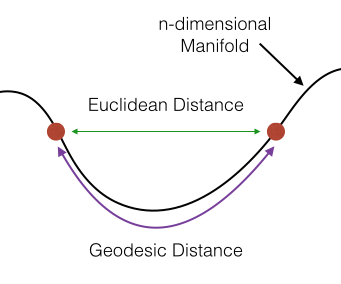
\includegraphics[width=0.5\textwidth]{Images/manifold-distance.png}	
	\caption{Diagram showing the difference between euclidean distance and geodesic distance between two points on a manifold.}
\end{figure}

Instead of using the euclidean distance metric (as in MDS) a weighted graph between all points is constructed. The geodesic distance between two points on the manifold is then given by the shortest path between two nodes in the graph. Typically this graph is constructed by finding the $k$ nearest neighbours of each datapoint and then using Dijkstra’s algorithm (or equivalent) to build the graph. Once the matrix of geodesic distances has been computed Isomap performs the same steps as classic MDS to achieve an embedding based on geodesic rather than euclidean distance.

One of the biggest issues with Isomap is ``short-circuiting". This is where the parameter $k$ for the number of nearest neighbours is set to be too large. In this case a point's $k$ largest neighbour may not be anywhere near the point's actual local neighbourhood resulting in a sub optimum lower dimensional representation.

\subsection{Locally Linear Embedding}
Locally linear embedding (LLE) \cite{roweis2000nonlinear} is another dimensionality reduction algorithm that is based on the principle of eigendecomposition but is substantially different in its approach. While Isomap focusses on the global structure of the embedded manifold locally linear embedding aims to preserve the local structure.

The fundamental assumption made by LLE is that the local neighbourhood surrounding a data point is roughly linear. Through this assumption LLE attempts to model each data point in terms of a matrix of weights required to ``recreate" a data point from its neighbours \cite{strange2014open}. 

LLE begins by finding each data point's $k$ nearest neighbours. From the local neighbours a cost function can be defined that yields the reconstruction error of the weights given by

\begin{equation}
	\epsilon(\bm{W}) = \sum\limits_i || \bm{x}_i - \bm{W}_{ij}\bm{x}_j ||^2 
\end{equation}

Where $\bm{W}_{ij} = 0$ if $\bm{x}_j$ is not in the local neighbourhood and $\sum\limits_j \bm{W}_{ij} = 1$ if it is. Minimising the weight matrix yields a least squares problem described in \cite{roweis2000nonlinear}. After obtaining the optimal weights for reconstructing the data point the matrix $\bm{W}$ can be used for find a lower dimensional representation by minimising the equivalent cost function for the lower dimensional space given by

 \begin{equation}
 	\Phi(\bm{Y}) = \sum\limits_i || \bm{y}_i - \bm{W}_{ij}\bm{y}_j ||^2 
 \end{equation}
 
 Subject to the constraints that the outputs are centred ($\sum\limits_j \bm{y}_i = 0$) and the outputs have unit covariance \cite{strange2014open}. Eigendecomposition of the feature matrix given by $\bm{F} = (\bm{I} - \bm{W})^T(\bm{I} - \bm{W})$  to obtain the bottom $d+1$ eigenvectors produces the desired embedding.
 
 LLE often produces better results than Isomap especially when the local structure of the embedded manifold is more important than the global structure. The optimisation of LLE is also quicker in comparison, largely due to it's ability to take advantage of sparse matrix algorithms. LLE can also have issues if the chosen neighbourhood is too large or if the density of the higher dimensional space is not uniform.

\section{Quality Measures}
\label{sec:quality-measures}
Performing dimensionality reduction on a dataset by definition causes a loss of information. As such, a lower dimensional embedding will always contain differences compared to the higher dimensional representation. The quality of the mapping produced by a dimensionality reduction algorithm can be measured by examining how the neighbourhood of a point in the higher dimensional data changes in the lower dimensional representation. In a good representation the neighbours in the higher dimensional space should be the same in the lower dimensional space.

One way of quantifying the quality of a mapping is by using measures derived from the co-ranking matrix \cite{lee2009quality}. Informally the co-ranking matrix is a square matrix representing the joint histogram of ranks between the two spaces. In this context the rank of data point $j$ is a number representing its position in the ordered list of data points sorted by distance from point $i$.

More formally the co-ranking matrix is given by the following definition. Let the higher dimensional dataset be denoted by $X = \{x_1, ..., x_n\} \subset \mathbb{R}^H$ and the lower dimensional set by $Y = \{y_1, ..., y_n\} \subset \mathbb{R}^L$. Let $\delta_{ij}$ denote the distance between the data point $i$ and $j$ in $\mathbb{R}^H$ and $d_{ij}$ the corresponding distance in $\mathbb{R}^L$. The rank of $x_j$ with respect to $x_i$ is given by

\begin{equation}
	\rho_{ij} = |\{k | \delta_{ik} < \delta_{ij} \lor (\delta_{ik} = \delta_{ij} \land 1 \leq k < j \leq N\}|
\end{equation}

Analogously the rank of $y_j$ with respect to $y_i$ is given by

\begin{equation}
	r{ij} = |\{k | d_{ik} < d_{ij} \lor (d_{ik} = d_{ij} \land 1 \leq k < j \leq N\}|
\end{equation}

The co-ranking matrix is then defined as the histogram of all rank errors $\bm{Q} = [q_{kl}]_{1 \leq k, l \leq N-1}$ where

\begin{equation}
	q_{kl} = |\{(i,j) | \rho_{ij} = k \land r_{ij} = l\}|
\end{equation}

In an idealised, perfect projection the co-ranking matrix would be a square diagonal matrix. However, because pairs of points will inevitably change their rank between the original representation and the projection errors in ranking will show up as off-diagonal entries in the matrix. A point whose rank decreases ($\rho_{ij} > d_{ij}$)  is called an intrusion. Conversely a point whose rank increases ($\rho_{ij} < d_{ij}$) is called an extrusion. A number of different weighted sums of the co-ranking matrix have been proposed which aim to measure the properties of the rank errors over local neighbourhoods of size $K$.

The co-ranking matrix may be further subdivided into four blocks based on the first $K$ rows and columns. Formally this is given by the cartesian product of the index sets $\mathbb{F}_K = \{1, .., K\}$ and $\mathbb{L}_K \{K+1, ..., N-1\}$ as follows:

\begin{align}
	\mathbb{UL}_K = \mathbb{F}_K \times \mathbb{F}_K,  \mathbb{UR}_K = \mathbb{F}_K \times \mathbb{L}_K
	\\
	\mathbb{LL}_K = \mathbb{L}_K \times \mathbb{F}_K,  \mathbb{LR}_K = \mathbb{L}_K \times \mathbb{L}_K
\end{align}

\begin{figure}
	\label{fig:co-ranking-matrix}
	\centering
	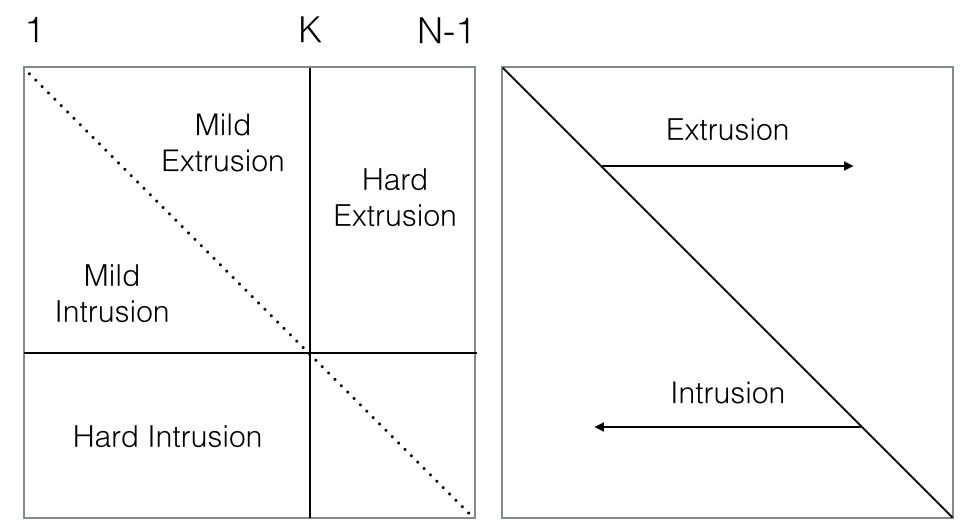
\includegraphics[width=0.8\textwidth]{Images/co-ranking.png}	
	\caption{Global structure of the co-ranking matrix. Trustworthiness measures hard intrusions and continuity measures hard extrusions in the lower left and upper right submatrix respectively. The local continuity meta-criteria measures the mild intrusion and extrusions in the upper left submatrix.}
\end{figure}


One set of measures which can be derived from the co-ranking matrix was suggested by Venna and Kaski \cite{kaski2003trustworthiness} is called the trustworthiness and continuity of the mapping. If a mapping is trustworthy the $k$ closest neighbours in the original space will be neighbours in the projected space. Specifically the trustworthiness metric measures how many points in the low dimensional neighbourhood are not in the high dimensional neighbourhood. In the context of the co-ranking matrix trustworthiness measures the ``hard" intrusions into the local neighbourhood corresponding to the lower left portion of the co-ranking matrix given by $\mathbb{LL_K}$. Another interpretation is to view this as measuring the number of true positives. The trustworthiness measure is defined in terms of the co-ranking matrix as \cite{lee2009quality}:

\begin{equation}
	T = 1 - \frac{2}{G_{K}} \sum\limits_{(k,l) \in \mathbb{LL}_K} (k - K)q_{kl}
\end{equation} 

Where $G_K$ is a normalising constant defined as

\begin{equation}
\label{eq:co-ranking-norm}
	G_K =
\left\{
	\begin{array}{ll}
		NK(2N - 3K - 1)  & \mbox{if } K < N \\
		N(N - K)(N - K - 1) & \mbox{if } K \geq N
	\end{array}
\right.
\end{equation}

On the other side of the coin the quality of a mapping can be degraded by discontinuity. Continuity is effectively the reverse of the trustworthiness measure. If the neighbours exist in the neighbourhood of the original space but not in the mapping then the nature of the original space may not be preserved due to discontinuities in the projection. In the context of the co-ranking matrix continuity measures the number of "hard" extrusions in the local neighbourhood which corresponds to the upper right proportion of the co-ranking matrix given by $\mathbb{UR_K}$. The measure of continuity in terms of the co-ranking matrix is given by \cite{lee2009quality}:

\begin{equation}
	C = 1 - \frac{2}{G_{K}} \sum\limits_{(k,l) \in \mathbb{UR}_K} (l - K)q_{kl}
\end{equation}

Where $G_K$ is the same as in equation \ref{eq:co-ranking-norm}.

Another measure proposed by Chen and Buja \cite{chen2009local} is the local continuity meta-criteria (LCMC). In contrast to the measures of trustworthiness and continuity which attempts to quantify the error in the projection the LCMC attempts to quantify how well the dimensionality reduction algorithm performed. The LCMC can be viewed as a measure of the true positives. In the context of the co-ranking matrix the LCMC is given by

\begin{equation}
	LCMC = \frac{K}{1 - N} + \frac{1}{NK} \sum\limits_{(k,l) \in \mathbb{UL}_K} q_{kl}
\end{equation}

One final measure that can be derived from the co-ranking matrix is the mean relative rank error (MMREs) proposed by Lee and Verleysen \cite{lee2007nonlinear}. The MRREs are similar to the measures of trustworthiness and continuity. While trustworthiness and continuity measure the ``hard"" intrusions and extrusions in a mapping, MRREs incorporate both ``mild" and ``hard" intrusions and extrusions. MRREs can be seen as quantifying both types of positives and negatives as opposed to trustworthiness and continuity only quantifying the false positives/negatives \cite{lee2009quality}. The MRREs are defined given in terms of the co-ranking matrix as

\begin{equation}
	W_n(K) = \frac{1}{H_k} \sum\limits_{(k,l) \in \mathbb{UL}_K \cup \mathbb{LL}_K} \frac{| k - l |}{l} q_{kl}
\end{equation}

\begin{equation}
	W_v(K) = \frac{1}{H_k} \sum\limits_{(k,l) \in \mathbb{UL}_K \cup \mathbb{UR}_K} \frac{| k - l |}{l} q_{kl}
\end{equation}

Where $H_k$ is the normalising factor given by

\begin{equation}
	H_k = N \sum\limits_{k=1}^K \frac{| N - 2k -1 |}{k}
\end{equation}

\section{Visualisation}
\label{sec:visualisation}
Traditionally plots of related low dimensional variables can be visualised directly using two or three dimensional scatterplots. However, direct visualisation of data with more than two or three dimensions is impossible with traditional methods. While dimensionality reduction techniques can be used to reduce the dimensionality of data down to two or three dimensions, it is often unlikely that two or three dimensions are enough to accurately capture the structure of a complex higher dimensional manifold.

While a higher dimensional dataset cannot be directly visualised in the traditional sense, several different visualisation techniques have been developed that can be used to examine the structure present in higher dimensional data. This sections provides a brief review of several of these techniques.

\subsection{Scatterplot matrix}

\begin{figure}[H]
	\label{fig:scatterplot-matrix}
	\centering
	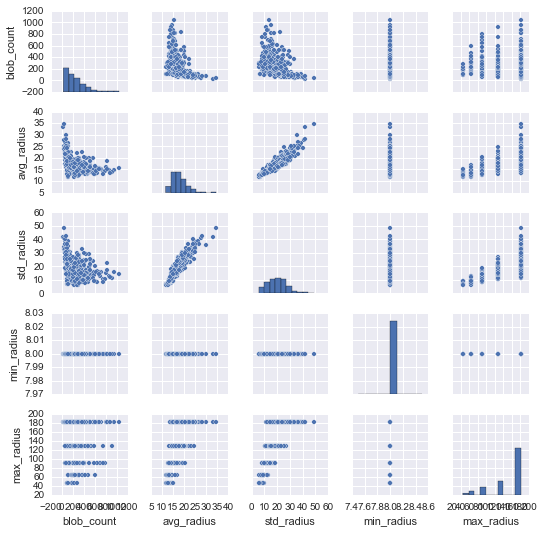
\includegraphics[width=0.5\textwidth]{Images/scatterplot-matrix.png}	
	\caption{An example of a scatter plot matrix showing the relationship between five different variables.}
\end{figure}

A scatterplot matrices are possibly the simplest form of higher dimensional plot. Traditional scatterplots show the relationship between two variables. A scatterplot matrix is an $n \times n$ matrix of scatterplots where each individual plot shows the correlation between two variables i.e. the plot in row $i$ and column $j$ will show the plot of variables $X_i$ and $X_j$  A downside to visualisation by scatterplot matrices is that an $n \times n$ matrix to visualise all dimensions. As the number of dimensions grows the number of subplots increases rapidly. This increases the time complexity required to generate the plot and the size of the screen space required to view it.

\subsection{Parallel Coordinates}

\begin{figure}[H]
	\label{fig:parallel-coords-plot}
	\centering
	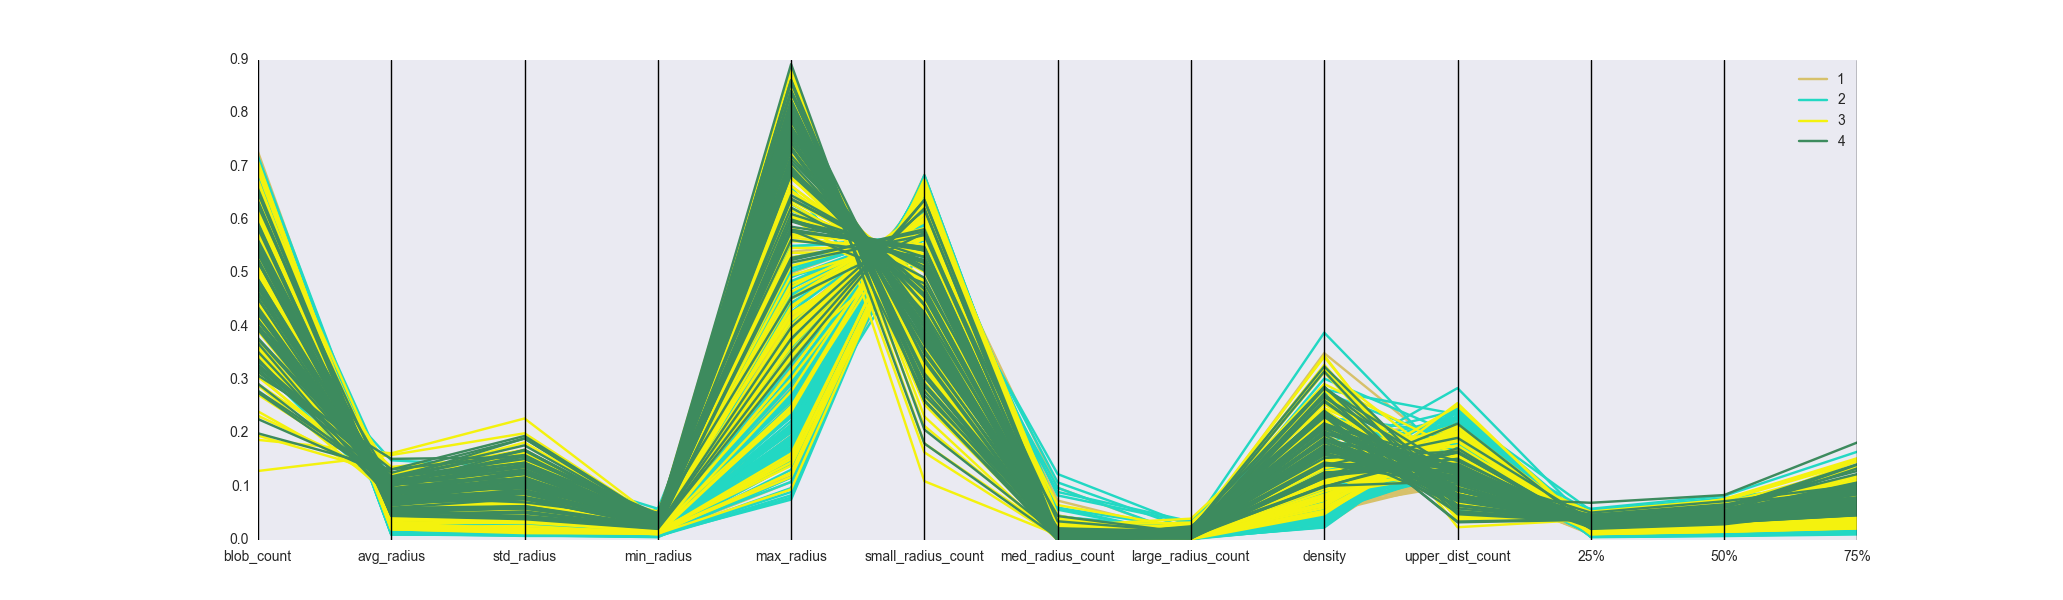
\includegraphics[width=1.0\textwidth]{Images/parallel-coords-plot.png}	
	\caption{An example of a parallel coordinate plot showing the relationship between a collection variables.}
\end{figure}

Parallel coordinate plots \cite{inselberg1991parallel} show each variable as a single axis along the bottom of the graph. A single point on the plot is represented as a piecewise line across each of the axes. The position at which a point intersects an axis is the value of that the $n$-dimensional data point has for that variable.

There are some limitations to parallel coordinate plots. The principle limitation is that the effectiveness of the visualisation is dependant on the ordering of the axes. Different orderings will produce different visualisations. Sometimes the data naturally has a specific ordering (such as time-series data), however this is often not the case. Tatu et al. \cite{tatu2009combining} experimented with using the Hough transform to automatically infer "good" axis orderings. Johansson et al \cite{johansson2009interactive} investigated ranking axis orderings using a combination of clustering, correlation and outlier features on the data. The scaling of each axis is also an important factor in the visualisation, however this can be solved by rescaling the data prior to visualisation.

\subsection{Andrews Plot}
An Andrews plot defines each $n$-dimensional data point as a Fourier series with $n$ terms. This visualisation is essentially the same as a parallel coordinates plot with each of the data points interpolated with Fourier interpolation. As such it suffers from the same limitations as parallel coordinates.

\begin{figure}[H]
	\label{fig:andrews-curve}
	\centering
	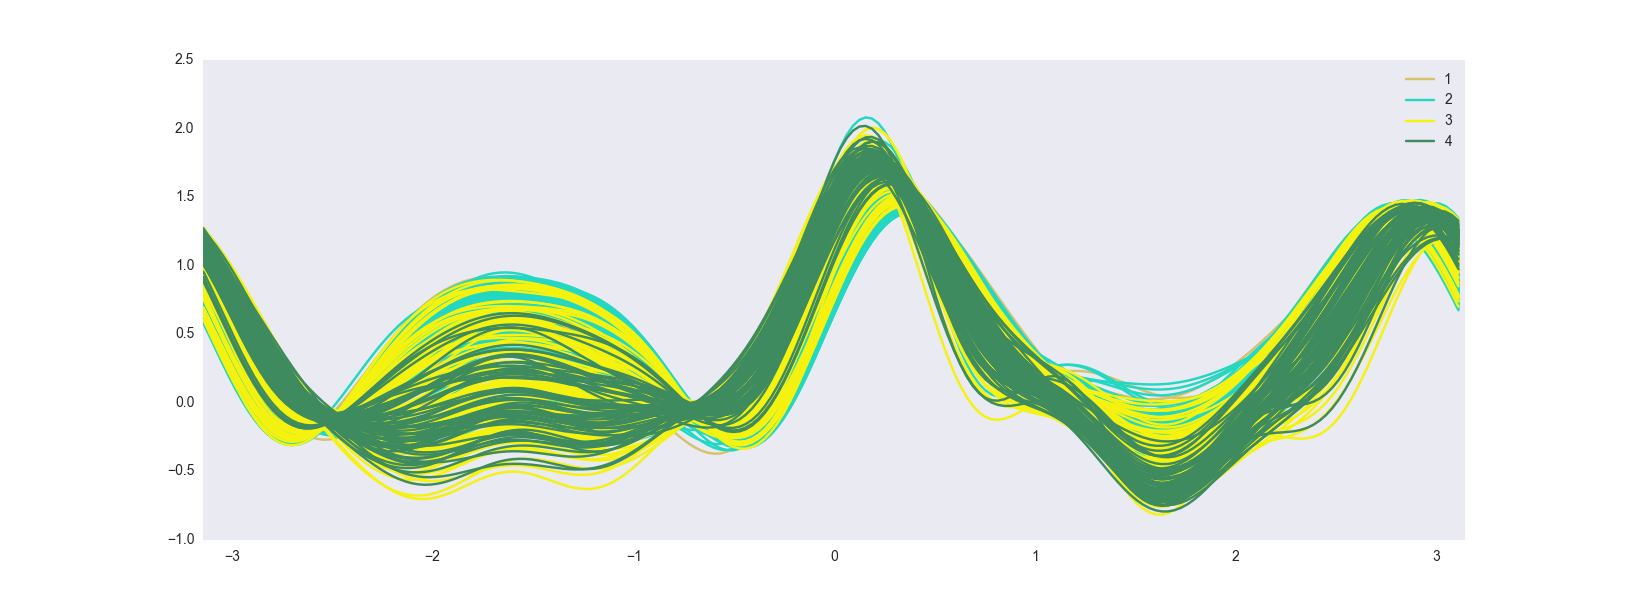
\includegraphics[width=1.0\textwidth]{Images/andrews-curve.png}	
	\caption{An example of a andrews curve plot showing the relationship between a collection variables.}
\end{figure}

\subsection{RadViz}

\begin{figure}[H]
	\label{fig:radviz-plot}
	\centering
	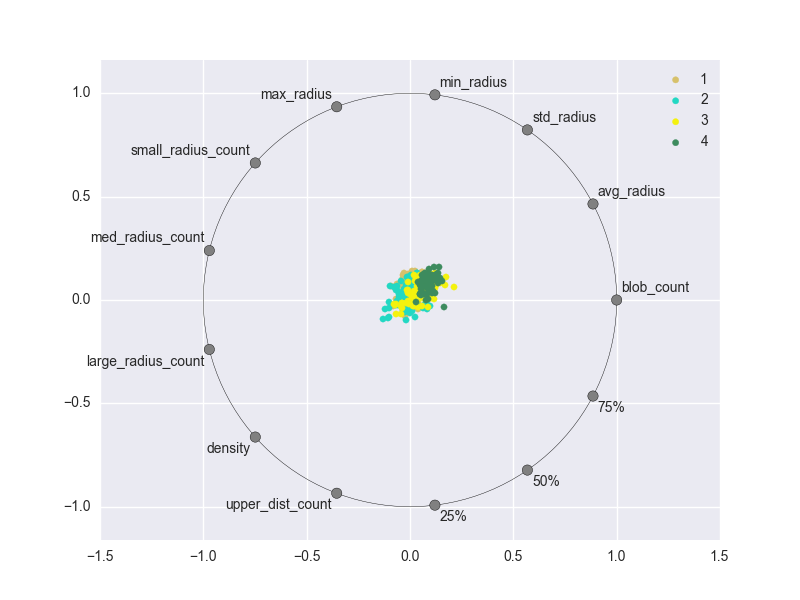
\includegraphics[width=0.7\textwidth]{Images/radviz-plot.png}	
	\caption{An example of a radviz plot showing the relationship between a collection variables.}
\end{figure}


RadViz \cite{novakova2009radviz} is a technique for visualising data points on a plane. RadViz models each $n$ dimensional data point as a single point on a 2D plane surrounded by a unit circle on which each of the $n$ features are placed equal distance apart from one another. Each data point is virtually ``connected" to each of the points on the unit circle via a ``spring". All of the springs are in equilibrium with one another and the final resting point for a point in the visualisation corresponds to the total strength exerted over point by each spring.

\section{Analysis}
This project aims to investigate the effect of mapping the feature space of both real and synthetic mammograms to a lower dimensional representation. This will involve the extraction of a variety of different shape, intensity, and texture features to produce a high dimensional feature space. We will then use dimensionality reduction techniques to produce a lower dimensional mapping and visualise the results using an appropriate technique. 

The hypothesis that we are aiming to test in the project is: Does the lower dimensional mappings of the higher dimensional feature space of synthetic mammograms match those of real patients? The high level questions that this project aims to answer are:

\begin{itemize}
	\item Are features which are important to real mammogram comparable to those of synthetic mammograms?
	\item If not, why are they different and does this relate to the author's own limitations?
	\item Can the knowledge gained be used to influence the perception of what features are important in a real mammogram?
	\item Could it be used to suggest how to build new mammogram models?
\end{itemize}

The technical work of the project will be concerned with implementing some existing approaches to feature extraction and dimensionality reduction in mammographic image analysis, but applying it to synthetic mammograms in order to evaluate the similarities and differences.

\begin{figure}
	\label{fig:pipeline-diagram}
	\centering
	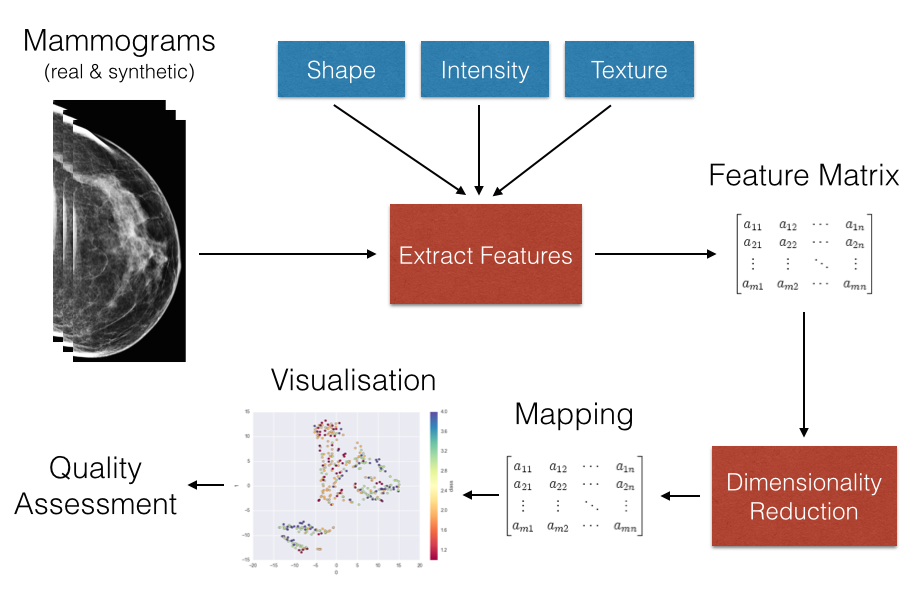
\includegraphics[width=0.8\textwidth]{Images/pipeline-diagram.png}	
	\caption{Conceptual overview of the image analysis pipeline to be produced as part of this project.}
\end{figure}

There are four core components of the methodology that need to be considered before implementation. The first is a decision on the number and type of features to be extracted from the images. Ideally the method used in this project should incorporate approaches that cover all three categories discussed in section \ref{sec:features}. This is so that a good variation in the types of approaches used will be incorporated into the system. Focussing on only one technique of extracting features considerably reduces the information that could be used to discriminate between images and risk classes. 

In this project, it is proposed that shape features are focussed on first. Due to the differences between real and synthetic mammograms, shape features are most likely to be the most successful for comparison between the two datasets. Then the focus will then sift to extracting intensity features and finally texture features. It is proposed that two shape features are used, one which detects blob features proposed by Chen et al. \cite{chen2013multiscale} and a linear structure feature proposed by Zwiggelaar et al. \cite{zwiggelaar1996finding}. Both of these techniques are fairly easy to interpret and are well understood by my supervisors. Regarding texture features those which are based on the GLCM \cite{haralick1973textural} are well tested and should be comparatively easy to get working. 

The second is the choice of dimensionality reduction techniques used to produce a lower dimensional mapping. Many different methods have been proposed for dimensionality reduction. It is highly likely relationship between variables in the feature space will not be a linear subspace. For this reason the chosen technique will almost certainly be a non-linear dimensionality reduction technique. However, it may be the case that the a linear dimensionality reduction technique such as PCA can be used to remove extremely redundant dimensions and reduce noise as a preprocessing step to a non-linear dimensionality reduction technique. 

t-SNE is a good choice for visualisation as it is specifically designed to find an embedding which are produce good clusters and preserves local neighbourhoods. However using just this one approach does not tell us anything about the global structure of the manifold on which the higher dimensional data lies. For understanding the global structure of the system it would be worth examining the projection created from a technique such as Isomap or locally linear embedding. All three of these are common dimensionality reduction approaches that are readily available in many languages and platforms (see section \ref{sec:choice-of-language}).

Thirdly the lower dimensional mapping must be visualised. This may be done either directly if the mapping is to two or three dimensions. Alternatively the a higher dimensional plot such as those discussed in section \ref{sec:visualisation} could be used to higher examine the dimensional spaces. The choice of visualisation techniques will depend heavily on the choice of the two prior components. It is likely that the project will use a combination of different visualisation strategies depending on what specific aspect of the dataset is being examined. One of the issues with higher dimensional data is that it is impossible to produce visualisation that accurately capture all aspects of the data at once. Whatever technique is used will only ever show a projection of the feature space at best.

The final component of the system will be a form of quality measurement. While visual examination of the mapping is a necessity for qualitatively interpreting how the mapping is derived from the feature space, it is important to gain a quantitive measurement of the mapping. Quantitive measures can be used to check parameters for the dimensionality reduction algorithm are well configured and compare can compare between different combinations of features. 

There will be two main results produced by this project. The first is an analysis of how well each of the features extracted and subsequent projections produced the phantom dataset match with those of the real mammogram dataset. The second is an analysis of the quality of the projections produced. This is important as it indicates whether the mapping is truly representative of the higher dimensional space. The part of the analysis will provide a statistical comparison of the feature spaces produced, the details of the test used described in section \ref{sec:comparison-of-features}. For checking the quality of the mappings produced we will use metrics based on the co-ranking matrix.

\subsection{Choice of Language}
\label{sec:choice-of-language}
A technical decision must also be made regarding the choice of technologies and programming languages to be used as part of the project. All four components of the system are likely to be non-trivial to implement. Where possible existing implementations of parts of the four major components of this project should be used. The reasons for this are threefold. 1) using existing implementations should ensure that the development time is kept to a minimum, 2) complex components are likely to be better tested for validity, and 3) there is no need to reinvent the wheel. 

The programming language used as part of the system must be capable of easily implementing high level operations. It would be useful if the language of choice readily includes high level libraries for image processing and dimensionality reduction as well as statistical packages. At the time of writing there are several contenders for potential language choices to be used in this project. 

Python \cite{pythonLanguage} is one of the more obvious choices. The language community has developed several useful libraries for image processing such as scikit-image \cite{van2014scikit} and OpenCV bindings \cite{openCV} as well as dimensionality reduction such as scikit-learn \cite{pedregosa2011scikit}. It also has lots of general purpose high level libraries likely to be useful in this project such as NumPy \cite{pythonNumpy}, Scipy \cite{jones2014scipy} and Pandas \cite{pythonPandas}. For visualisation the matplotlib library seems like an obvious choice. An additional strength of python it is a very high level language that is perfect for rapid prototyping. The programmer does not need to concern themselves with the manual memory management or type system as in C, C++ or Java. However, this does not necessarily come with a loss in performance. Libraries such as Numpy and Scipy provide extremely quick pre-compiled high level operations written in C, allowing us to join performance with simplicity.

A strong alternative contender to Python is the R language \cite{rlanguage}. R was originally designed as a statistical programming language but has good support for many of the requirements of this project. Like Python, R is a very high level scripting language which has many additional packages that can be installed such as packages for PCA \cite{rPCA}, t-SNE \cite{rtSNE}, LLE \cite{rLLE} etc. It also has the RIPA (R Image Processing and Analysis module) library for image processing \cite{rRIPA}. For visualisation the excellent ggplot2 \cite{rggplot2} library is a clear candidate for this language.

Alternative languages which could be appropriate for this project include Matlab and C++. Like R and Python Matlab \cite{matlab} is a relatively high level language which has an extensive collection of libraries for data analysis and visualisation as well as support for image processing. However, the major downside to the Matlab application is that it is not free, even on a student license. The performance and object orientation offered by C++ are the major benefits offered and has direct support of the OpenCV library. However, as mentioned above the major downside C++ is the headaches of manual memory management and type system.

In summary, I believe that the best choice of language for this project would be the Python programming language. This language combines the high level of abstraction that will be useful in this sort of project with performance that exceeds others such as R \cite{morandat2012evaluating}. The author's own intermediate level knowledge of Python is also a key factor here. The author's lack of personal experience with R and Matlab would be a severe hindrance this project. The Scipy stack is also an important factor. As many of the libraries that would be used in this project are made by the same developers there is a certain guarantee that the libraries will play well together, leading to less integration issues. As mentioned C++, while providing excellent performance, would not be such a good choice compared to Python because of the resulting implementation difficulties.

\section{Development Methodology}
The methodology for the implementation of the project will draw core on ideas from the agile development methodology. This software development methodology is the only one which makes sense for a research orientated project. Research orientated projects are by definition exploratory in nature and the results of the project cannot be stated in concrete at the start of the project. This rules out methodologies like waterfall and feature driven because in both systems the end result of development must be clearly stated up front, with little room for manoeuvre.

Agile approaches embrace change. This is a desirable attribute in a project where we can define the high level end goals of development but where the specifics must be flexible towards finding an approach that works based on analysis of the results from initial prototyping.

As this project is an individual endeavour the full power of an agile approach cannot be fully realised because some of the core principles rely on interactions between multiple individuals (such as daily stand-up meetings and paired programming from XP).

There are however many other benefits to an agile approach that are relevant to an individual project. Test driven development (TDD) is a concept that is highly relevant. In software development TDD is used to ensure that you have confidence to make changes and verification that what you have written works. This is especially relevant and desirable in research projects because it not only gives you verification that the software is working, but can also be used to verify that the output of the program and therefore results are correct.

Short iterations and small releases that incrementally add value is another concept that is relevant to an individual project. This provides a measurable indicator of progress throughout the project. This project will aim to produce weekly iterations which will select several stories to work on throughout the week. The start of an iteration will be timed to coincide with the meeting with the postdoc supervisor who will effectively act as a ``customer" to the project. Work for the week will be decided based on discussions during these meetings so this naturally defines an anchor for iteration beginnings and endings.

Programmatic idioms associated with XP are also of value to an individual project. Simplicity (especially the concept of YAGNI) and heavy refactoring are likely to feature heavily in this project. Simplicity ensures that we keep the focus of the project limited to the goals of the research question without adding superfluous code that doesn't contribute to answering the questions outlined the problem analysis. Refactoring will allow the design of the project to be incremental. We can start with an initial basic design and rewrite and modify the structure of the code when it is needed in order to accommodate problems encountered or other change. In this way a good design (where verification of correctness is controlled by TDD) becomes a natural byproduct of development.

The methodology used will also heavily utilise version control. Git will be used as the version control for the code base created during this project and a copy of the code will be stored remotely on the Github website. As part of the process used in this project, new features will be developed on branches from the existing master, tested on the build server and finally integrated into the system as a whole.


